%% abtex2-modelo-trabalho-academico.tex, v<VERSION> laurocesar
%% Copyright 2012-<COPYRIGHT_YEAR> by abnTeX2 group at http://www.abntex.net.br/ 
%%
%% This work may be distributed and/or modified under the
%% conditions of the LaTeX Project Public License, either version 1.3
%% of this license or (at your option) any later version.
%% The latest version of this license is in
%%   http://www.latex-project.org/lppl.txt
%% and version 1.3 or later is part of all distributions of LaTeX
%% version 2005/12/01 or later.
%%
%% This work has the LPPL maintenance status `maintained'.
%% 
%% The Current Maintainer of this work is the abnTeX2 team, led
%% by Lauro César Araujo. Further information are available on 
%% http://www.abntex.net.br/
%%
%% This work consists of the files abntex2-modelo-trabalho-academico.tex,
%% abntex2-modelo-include-comandos and abntex2-modelo-references.bib
%%

% ------------------------------------------------------------------------
% ------------------------------------------------------------------------
% abnTeX2: Modelo de Trabalho Academico (tese de doutorado, dissertacao de
% mestrado e trabalhos monograficos em geral) em conformidade com 
% ABNT NBR 14724:2011: Informacao e documentacao - Trabalhos academicos -
% Apresentacao
% ------------------------------------------------------------------------
% ------------------------------------------------------------------------

\documentclass[
	% -- opções da classe memoir --
	12pt,				% tamanho da fonte
	openright,			% capítulos começam em pág ímpar (insere página vazia caso preciso)
	twoside,			% para impressão em recto e verso. Oposto a oneside
	a4paper,			% tamanho do papel. 
	% -- opções da classe abntex2 --
	%chapter=TITLE,		% títulos de capítulos convertidos em letras maiúsculas
	%section=TITLE,		% títulos de seções convertidos em letras maiúsculas
	%subsection=TITLE,	% títulos de subseções convertidos em letras maiúsculas
	%subsubsection=TITLE,% títulos de subsubseções convertidos em letras maiúsculas
	% -- opções do pacote babel --
	english,			% idioma adicional para hifenização
	french,				% idioma adicional para hifenização
	spanish,			% idioma adicional para hifenização
	brazil,				% o último idioma é o principal do documento
	sumario=tradicional
	]{abntex2}

% ---
% Carregando pacotes necessários para gerar o PDF 
% ---
% ---
% Pacotes básicos 
% ---
\usepackage{lmodern}		% Usa a fonte Latin Modern			
\usepackage[T1]{fontenc}	% Selecao de codigos de fonte.
\usepackage[utf8]{inputenc}	% Codificacao do documento (conversão automática dos acentos)
\usepackage{lastpage}		% Usado pela Ficha catalográfica
\usepackage{indentfirst}	% Indenta o primeiro parágrafo de cada seção.
\usepackage{color}			% Controle das cores
\usepackage{xcolor}			% Controle das cores
\usepackage{graphicx}		% Inclusão de gráficos
\usepackage{microtype} 		% para melhorias de justificação
% ---
% Adicionado por Madson Dias
% ---

\graphicspath{ {figuras/graficos/} {figuras/imagens/}}  % Inclusão dos paths para imagens
\usepackage{xstring} 	% Criar comandos com IF
\usepackage{caption}
\usepackage{subcaption}
\usepackage{mdframed}
\usepackage{microtype}
\usepackage{pdfpages}
\usepackage{listings}
\usepackage{textcomp}
\usepackage{float}
\usepackage{chngcntr}		% Criar numeração de imagens por capítulo
\counterwithin{figure}{section}
\usepackage[os=win]{menukeys}
\usepackage{multicol}
\usepackage{framed}
% \usepackage{helvet}
% \usepackage{geometry}
% \usepackage{marginnote}

% ---
% Pacotes adicionais, usados apenas no âmbito do Modelo Canônico do abnteX2
% ---
\usepackage{lipsum}				% para geração de dummy text
% ---

% ---
% Pacotes de citações
% ---
\usepackage[brazilian,hyperpageref]{backref}	 % Paginas com as citações na bibl
\usepackage[alf]{abntex2cite}	% Citações padrão ABNT

% --- 
% CONFIGURAÇÕES DE PACOTES
% --- 

% ---
% Configurações do pacote backref
% Usado sem a opção hyperpageref de backref
\renewcommand{\backrefpagesname}{Citado na(s) página(s):~}
% Texto padrão antes do número das páginas
\renewcommand{\backref}{}
% Define os textos da citação
\renewcommand*{\backrefalt}[4]{
	\ifcase #1 %
		Nenhuma citação no texto.%
	\or
		Citado na página #2.%
	\else
		Citado #1 vezes nas páginas #2.%
	\fi}%
% ---

% ---
% Alterando espaçamento dos itens
% ---
\setlist[itemize]{noitemsep, topsep=0pt, leftmargin=1.75cm}
\setlist[enumerate]{noitemsep, topsep=0pt, leftmargin=1.75cm}
\setlist[description]{noitemsep, topsep=0pt, leftmargin=1.75cm}

% ---
% Alterando o aspecto da cor azul
% ---
\definecolor{blue}{RGB}{41,5,195}

% --- 
% Espaçamentos entre linhas e parágrafos 
% --- 

% O tamanho do parágrafo é dado por:
\setlength{\parindent}{1.3cm}

% Controle do espaçamento entre um parágrafo e outro:
\setlength{\parskip}{0.2cm}  % tente também \onelineskip

\usepackage{utils/ejovem-modelo} 	% Pacote com informações da customização
\usepackage{utils/ejovem-programacao-web} 	% Pacote com informações da customização

% ---
% Informações de dados para FOLHA DE ROSTO
% ---
% Informações do Autor e do trabalho
% ------------------------------------
\autor{<Nome do Autor>}
\titulo{<Título da Dissertação>}
\area{<Área de Concentração>}

\orientador{<Nome do Orientador>}
\coorientador{<Nome do Coorientador>} % Se você tem um coorientador, descomente esta linha

% Professores convidados para a banca
% ------------------------------------
% 
%  - Caso tenha um terceiro professor convidado, remova os comentários

\nomeprofessorA{<Nome do Professor A>}
\instituicaoprofessorA{<Instituição do Professor A> (<Sigla A>)}

\nomeprofessorB{<Nome do Professor B>}
\instituicaoprofessorB{<Instituição do Professor B> (<Sigla B>)}

%\nomeprofessorC{<Nome do Professor C>}
%\instituicaoprofessorC{<Instituição do Professor C> (<Sigla C>)}

% ---
% Informações do PDF
% ---
\makeatletter
\hypersetup{
     	%pagebackref=true,
		pdftitle={\@title}, 
		pdfauthor={\@author},
    	pdfsubject={\imprimirpreambulo},
	    pdfcreator={LaTeX with abnTeX2},
		pdfkeywords={abnt}{latex}{abntex}{abntex2}{apostila}, 
		colorlinks=true,       		% false: boxed links; true: colored links
    	linkcolor=blue,          	% color of internal links
    	citecolor=blue,        		% color of links to bibliography
    	filecolor=magenta,      		% color of file links
		urlcolor=blue,
		bookmarksdepth=4
}
\makeatother
% --- 

% ---
% compila o indice
% ---
\makeindex
% ---

% ----
% Início do documento
% ----
\begin{document}

% Seleciona o idioma do documento (conforme pacotes do babel)
%\selectlanguage{english}
\selectlanguage{brazil}

% Retira espaço extra obsoleto entre as frases.
\frenchspacing 

% ----------------------------------------------------------
% ELEMENTOS PRÉ-TEXTUAIS
% ----------------------------------------------------------
% \pretextual
\imprimircapa % Capa *

% inserir lista de ilustrações
% \pdfbookmark[0]{\listfigurename}{lof}
% \listoffigures*
% \cleardoublepage
% inserir lista de tabelas
% \pdfbookmark[0]{\listtablename}{lot}
% \listoftables* \cleardoublepage
% ---
\setlength{\absparsep}{18pt} % ajusta o espaçamento dos parágrafos do resumo
\begin{resumo}
 Segundo a \citeonline[3.1-3.2]{NBR6028:2003}, o resumo deve ressaltar o
 objetivo, o método, os resultados e as conclusões do documento. A ordem e a extensão
 destes itens dependem do tipo de resumo (informativo ou indicativo) e do
 tratamento que cada item recebe no documento original. O resumo deve ser
 precedido da referência do documento, com exceção do resumo inserido no
 próprio documento. (\ldots) As palavras-chave devem figurar logo abaixo do
 resumo, antecedidas da expressão Palavras-chave:, separadas entre si por
 ponto e finalizadas também por ponto.

 \textbf{Palavras-chave}: latex. abntex. editoração de texto.
\end{resumo}  	% Apresentação do programa e-jovem 
\begin{siglas}
  \item[ABNT] Associação Brasileira de Normas Técnicas
  \item[abnTeX] ABsurdas Normas para TeX
  \item[PHP] Pré-Processador de Hipertexto
\end{siglas}  			% Lista de abreviaturas e siglas
% \begin{simbolos}
\item[$ \Gamma $] Letra grega Gama
\item[$ \Lambda $] Lambda
\item[$ \zeta $] Letra grega minúscula zeta
\item[$ \in $] Pertence
\end{simbolos} 				% Lista de símbolos

% inserir o sumario
\pdfbookmark[0]{\contentsname}{toc}
\tableofcontents*
\cleardoublepage
% ---



% ----------------------------------------------------------
% ELEMENTOS TEXTUAIS
% ----------------------------------------------------------
\textual

% ---
% PHP 
% ---
\chapter{\php}
% ---

Ao final deste capítulo, o aluno terá as seguintes competências:
\begin{enumerate}
	\item Entender a arquitetura cliente-servidor;
	\item Instalar o servidor web (nginx) e a linguagem \php; e
	\item Testar o ambiente de desenvolvimento. 
\end{enumerate}

\section{\phpcompleto}

O \phpcompleto, foi criado por \phpcriador~ em 1995 e originalmente chamado de 
“\textit{Personal Home Page Tools}” (Ferramentas para Página Pessoal). Com a 
aceitação do projeto, muitos programadores passaram a utilizar e propor mudanças,
surgindo assim, o \php~ que iremos conhecer hoje. O \php~ está atualmente na
versão 7.0, chamado de \php7 ou, simplesmente de \php. A nível de estudo, 
utilizaremos o \php~ \phpversao, pois é uma versão mais estável e muito 
utilizada no mercado.

O \php~ é uma linguagem de programação que funciona no lado do servidor, 
ele permite criarmos \sites dinâmicos, ou seja, o \site se comporta de acordo 
com a entrada de dados do usuário. Outros exemplos de linguagem semelhantes são 
ASP, JSP (Java) e Python.

A linguagem \php~ trabalha lado a lado com o \htmlcompleto, por conta disso vamos
precisar saber o básico de \html, principalmente as \tags~ de formulário. Devemos
lembrar que o \php~ tem pouca relação com o \layout~ ou eventos que compõem a 
aparência de uma página \web. Portanto, podemos dizer que a maior parte do que o
\php realiza é invisível para o usuário final. O internauta, ao visualizar a 
página desenvolvida em \php não será capaz de identificar que a página foi 
escrita utilizando a tecnologia disponibilizada pelo \php. 

Você arriscaria dizer que o Facebook foi desenvolvido com a linguagem \php?

\section{Arquitetura cliente-servidor}
\label{arquitetura-cliente-servidor}

Como visto na seção anterior, o \php~ funciona do lado do servidor. Para entendermos
melhor isso, é necessário entender a estrutura cliente/servidor. Muito utilizada
na \internet. A figura abaixo exemplifica de maneira simples a comunicação entre
cliente e servidor.

FIGURA

....

\section{Instalação do \php}
\label{instalacao-do-php}

Para que possamos utilizar o \php, devemos instalar a linguagem no nosso computador
de trabalho. Vamos instalar esses pacotes através do \terminal. Podemos abrir o
\terminal de várias maneiras. Veja duas delas listadas abaixo:

\begin{enumerate}
	\item clique com o botão direito na área de trabalho e escolha a a opção
	"Abra o Emulador de Terminal aqui"; e
	\item acione a combinação de teclas ALT + F2 e digite \xfceterminal.
\end{enumerate}

Em seguida escreva o comando abaixo no \terminal~ que acabamos de abrir. Por segurança
a senha de usuário será requisitada, e \textbf{ela não aparece ao ser digitada}.
Não se preocupe, digite a senha e ao final aperte enter. 

\begin{lstlisting}[language=bash, style=Comandos]
  $ sudo apt-get install php5 libapache2-mod-php5 php5-gd curl 
  	php5-curl php5-xmlrpc php5-cli
\end{lstlisting}

Se você estiver usando o Linux do Projeto e-Jovem, então esses pacotes já devem
ter sido instalados e você visualizou a seguinte tela.

\figurasimples{php-instalacao-ok}{Instalação do \php~ bem sucedida.}

\section{Instalação do \apache}
\label{instalacao-do-apache}

O servidor \apache~ é um dos principais aplicativos que fazem a \web~ funcionar.
Ele é responsável por interpretar os arquivos \phpextensao~ e retornar para o
cliente, apenas o que ele requisitou. A versão que vamos trabalhar é a \apacheversao.
O processo de instalação é parecido com o que foi utilizado no \php. Abra o
\terminal~ utilizando um dos passos da seção \ref{instalacao-do-php}.

\begin{lstlisting}[language=bash, style=Comandos]
  $ sudo apt-get install apache2
\end{lstlisting}

Se o sistema utilizado for o Linux do Projeto e-Jovem, então já temos o \apache
\apacheversao~ instalado (figura \ref{apache-instalacao-ok}). Digite no navegador 
Firefox o endereço de internet \url{http://localhost}. A tela será parecida com 
a mostrada na figura \ref{apache-verificacao-ok}.

\figuradupla{apache-instalacao-ok}{Instalação do \apache \apacheversao~ bem sucedida}
			{apache-verificacao-ok}{Verificação do \apache~ em execução. Digite \url{http://localhost} no navegador Firefox}

A figura \ref{apache-verificacao-ok} indica que o \apache~ está funcionando corretamente.
O arquivo apresentado acima pode ser encontrado no diretório \dirpadrao. Será 
essa a localização dos arquivos que vamos desenvolver. Ou seja, sempre que criarmos
um arquivo \phpextensao~ ele deverá ser salvo no \dirpadrao. 

Para que seja possível o usuário do sistema (no caso você) salve no \dirpadrao,
precisamos mudar a permissão de escrita do diretório. Vamos abrir o \terminal~
de acordo com o que foi mostrado na seção \ref{instalacao-do-php}. Com o \terminal~
aberto, digite o seguinte comando.

\begin{lstlisting}[language=bash]
  $ sudo chmod -R 777 /var/www 
\end{lstlisting}

O comando acima permite que o usuário comum do sistema grave arquivos no \dirpadrao.

O aplicativo \apache~ pode ser configurado para funcionar de diversas maneiras. 
Essa disciplina necessita apenas da configuração básica. Caso queira modificá-la, 
o aluno poderá ler mais sobre o \apache~ através do site: \url{http://httpd.apache.org/docs/2.2}.

Caso você use o sistema operacional Windows na sua casa, veja no apêndice 
TAL, lá é explicado como instalar o \php~ e o \apache~ no Windows.


\section{Testando o ambiente}
\label{testando-ambiente}

Após a instalação, devemos testar o nosso ambiente de desenvolvimento (composto
inicialmente por \php~ e \apache). Abra novamente o \terminal~, navegue até o
diretório \dirpadrao. 				% Capítulo 1 - PHP
\chapter{Lorem ipsum dolor sit amet}\label{cap:exampleChapter}
% ---
\section{Aliquam vestibulum fringilla lorem}
% ---

\lipsum[1]

% Exemplo de inclusão de figura
\begin{figure}[h]\label{fig:logo-ifce-sem-nome}
	\begin{center}
		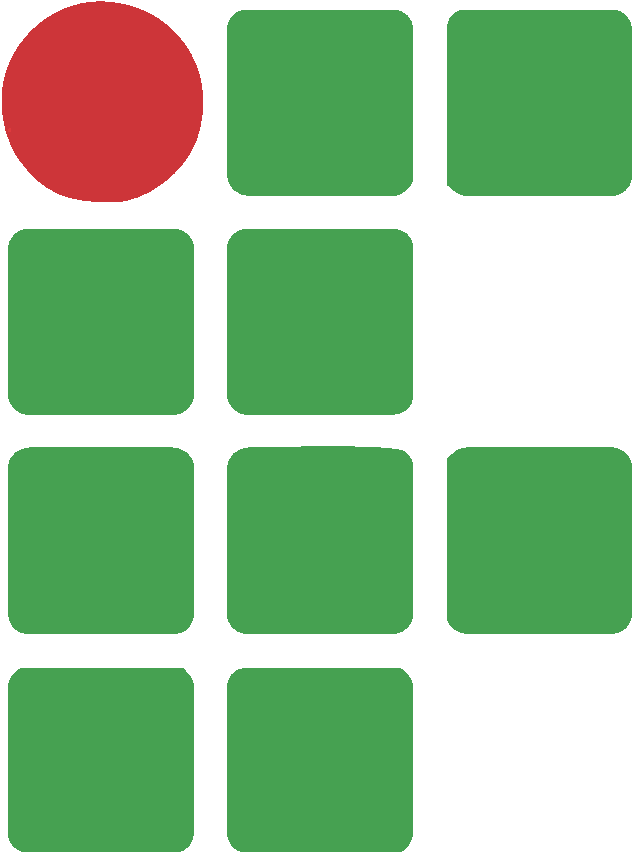
\includegraphics[width=4cm]{logo-ifce-sem-nome}
		\caption{Logomarca do IFCE sem nome}
	\end{center}
\end{figure}
% ------
\lipsum[2-3]

\includetable{tabela-exemplo} % Exemplo de inclusão de tabela

\lipsum[2-3]
% Exemplo de inclusão de gráficos
\begin{figure}
    \centering
    \begin{subfigure}[b]{0.45\textwidth}
        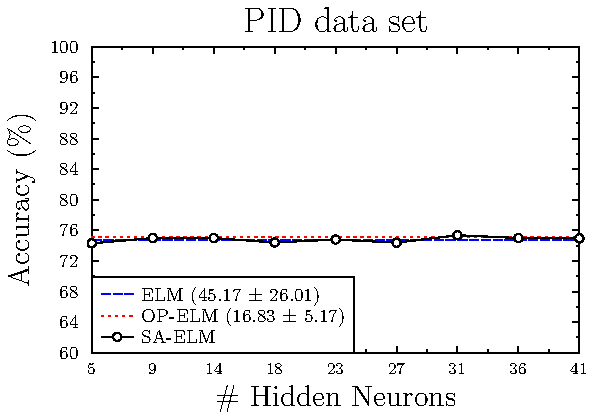
\includegraphics[width=\textwidth]{pid}
        \caption{Base de dados PID}
        \label{fig:pid}
    \end{subfigure}
    ~ 
    \begin{subfigure}[b]{0.45\textwidth}
        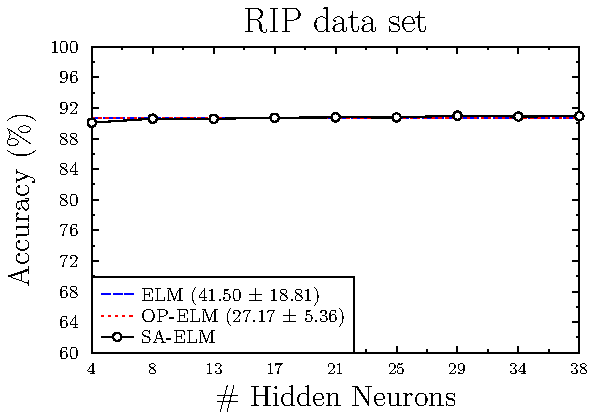
\includegraphics[width=\textwidth]{rip}
        \caption{Base de dados RIP}
        \label{fig:rip}
    \end{subfigure}
    \caption{Exemplo de gráfico}\label{fig:animals}
\end{figure}
% ------
\lipsum[1] 			% Capitulo de exemplo

% ----------------------------------------------------------
% Finaliza a parte no bookmark do PDF
% para que se inicie o bookmark na raiz
% e adiciona espaço de parte no Sumário
% ----------------------------------------------------------
\phantompart

% ---
% Conclusão
% ---
\chapter{Conclusão}
% ---

\lipsum[31-33] 				% Capítulo de introdução

% ----------------------------------------------------------
% ELEMENTOS PÓS-TEXTUAIS
% ----------------------------------------------------------
\postextual
% ----------------------------------------------------------

% ----------------------------------------------------------
% Referências bibliográficas
% ----------------------------------------------------------
\bibliography{referencias}

% ----------------------------------------------------------
% Glossário
% ----------------------------------------------------------
%
% Consulte o manual da classe abntex2 para orientações sobre o glossário.
%
%\glossary

% ----------------------------------------------------------
% Apêndices
% ----------------------------------------------------------

% ---
% Inicia os apêndices
% ---
\begin{apendicesenv}

% Imprime uma página indicando o início dos apêndices
\partapendices
% Insere os apêndices
% ----------------------------------------------------------
\chapter{Instalação de ambiente de desenvolvimento no Windows}
\label{ap:instalacao-env-windows}
% ----------------------------------------------------------
\lipsum[55-57]
\chapter{Quisque libero justo}
% ----------------------------------------------------------

\lipsum[50]
%\include{apendices/apendice-c}
%\include{apendices/apendice-d}




\end{apendicesenv}
% ---


% ----------------------------------------------------------
% Anexos
% ----------------------------------------------------------

% ---
% Inicia os anexos
% ---
\begin{anexosenv}

% Imprime uma página indicando o início dos anexos
\partanexos
% Insere os anexos
\chapter{Morbi ultrices rutrum lorem.}
% ---
\lipsum[30]

\chapter{Cras non urna sed feugiat cum sociis natoque penatibus et magnis dis
parturient montes nascetur ridiculus mus}
% ---

\lipsum[31]
%\include{anexos/anexo-c}
%\include{anexos/anexo-d}

\end{anexosenv}

%---------------------------------------------------------------------
% INDICE REMISSIVO
%---------------------------------------------------------------------
\phantompart
\printindex
%---------------------------------------------------------------------

\end{document}
